Se comparan seis representaciones con receptor independiente: imagen original, \texttt{resize\_16x16}, \texttt{resize\_8x8}, \emph{embedding}, etiqueta y silencio. La corrida principal usa Fashion-MNIST completo, 5 \'epocas, 3 semillas y backend \texttt{torch}. La Tabla 1 resume los resultados.

\begin{table}[t]
\centering\small
\caption{Fase 1 (Fashion-MNIST). Exactitud media $\pm$ desviaci\'on est\'andar entre 3 semillas.}
\begin{tabular}{@{}lrrrr@{}}
\toprule
Representaci\'on & Bytes & Exactitud & Utilidad/byte & Ahorro\\
\midrule
original (PNG)        & 512{,}4 & 0{,}8895 $\pm$ 0{,}0016 & 0{,}00174 & ---\\
resize $16{\times}16$ & 212{,}3 & 0{,}8577 $\pm$ 0{,}0038 & 0{,}00404 & 58{,}6\%\\
resize $8{\times}8$   &  78{,}8 & 0{,}7894 $\pm$ 0{,}0052 & 0{,}01002 & 84{,}6\%\\
\textbf{embedding}    &  \textbf{50{,}4} & \textbf{0{,}8925 $\pm$ 0{,}0028} & \textbf{0{,}01771} & \textbf{90{,}2\%}\\
etiqueta              &  21{,}0 & 0{,}8876 $\pm$ 0{,}0030 & 0{,}04227 & 95{,}9\%\\
silencio              &   0{,}0 & 0{,}1000 & --- & 100\%\\
\bottomrule
\end{tabular}
\end{table}

\begin{figure}[t]
\centering
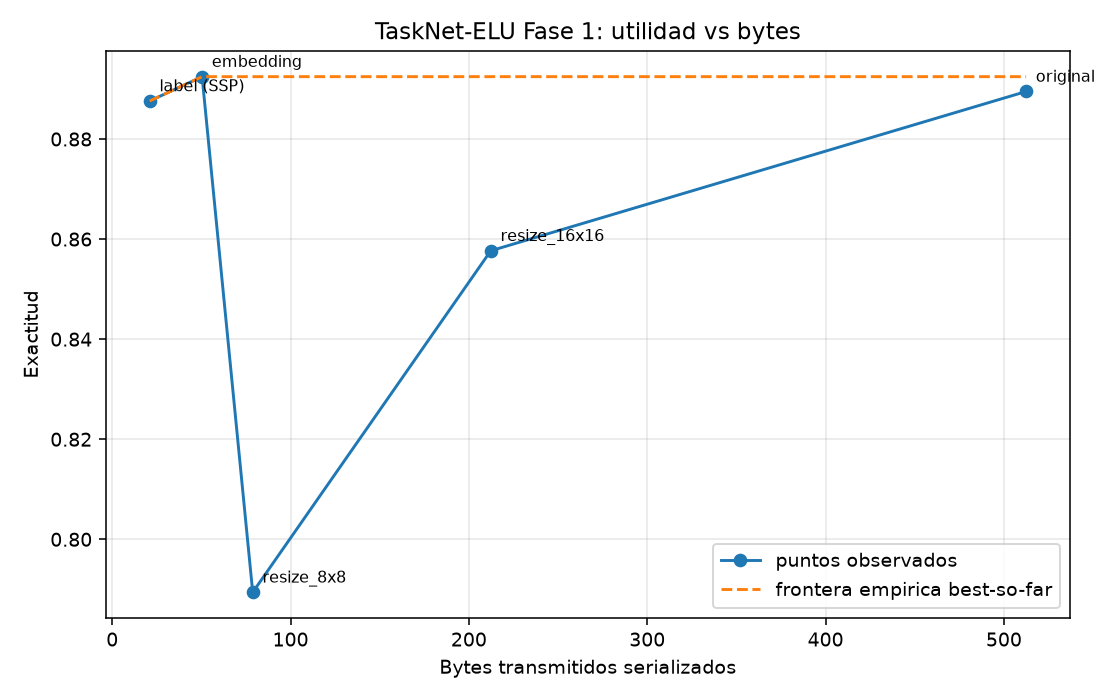
\includegraphics[width=0.82\linewidth]{results/figures/accuracy_vs_bytes.png}
\caption{Fase 1: utilidad vs. bytes en Fashion-MNIST. Los puntos emp\'iricos observados no tienen por qu\'e ser mon\'otonos; la lectura relevante es la envolvente/frontera emp\'irica entre utilidad y bytes.}
\end{figure}

\textbf{Lectura.} El \emph{embedding} es el SSP sem\'antico dentro del cat\'alogo evaluado: conserva la utilidad del dato completo con 90{,}2\% menos bytes. La etiqueta aparece como SSP general/de decisi\'on porque representa una decisi\'on ya tomada; no es una representaci\'on sem\'antica reutilizable y no debe tratarse como equivalente al \emph{embedding}. No aparece SSP visual: las reducciones de imagen no conservan utilidad con ahorro suficiente. Un punto relevante es que \texttt{resize\_8x8} pesa m\'as que el \emph{embedding} (78{,}8 vs. 50{,}4 bytes) y obtiene bastante menos exactitud. Es decir, los puntos observados no siguen una relaci\'on mon\'otona simple: m\'as bytes no implican autom\'aticamente m\'as utilidad. Bajo esta tarea, la organizaci\'on de la informaci\'on en la representaci\'on pesa m\'as que el tama\~no bruto.

% ==========================================================
\section{Fase 2: representaci\'on aprendida vs. compresi\'on cl\'asica}

La Fase 2 compara el \emph{embedding} contra PNG, JPEG a calidades $\{90,50,20,10,5\}$ y reducciones de resoluci\'on, todas evaluadas con receptores independientes entrenados sobre las representaciones reconstruidas. La corrida usa Fashion-MNIST completo, 5 \'epocas y 3 semillas. La Tabla 2 y la Figura 2 resumen los resultados principales.

\begin{table}[t]
\centering\small
\caption{Fase 2 (Fashion-MNIST), filas seleccionadas.}
\begin{tabular}{@{}lrrr@{}}
\toprule
Representaci\'on & Bytes & Exactitud & Utilidad/byte\\
\midrule
original (PNG)        & 512{,}5 & 0{,}8859 & 0{,}00173\\
JPEG q90              & 742{,}9 & 0{,}8851 & 0{,}00119\\
JPEG q5               & 383{,}5 & 0{,}8622 & 0{,}00225\\
resize $8{\times}8$   &  78{,}8 & 0{,}7984 & 0{,}01014\\
\textbf{embedding}    & \textbf{50{,}4} & \textbf{0{,}8916} & \textbf{0{,}01769}\\
\bottomrule
\end{tabular}
\end{table}

\begin{figure}[t]
\centering
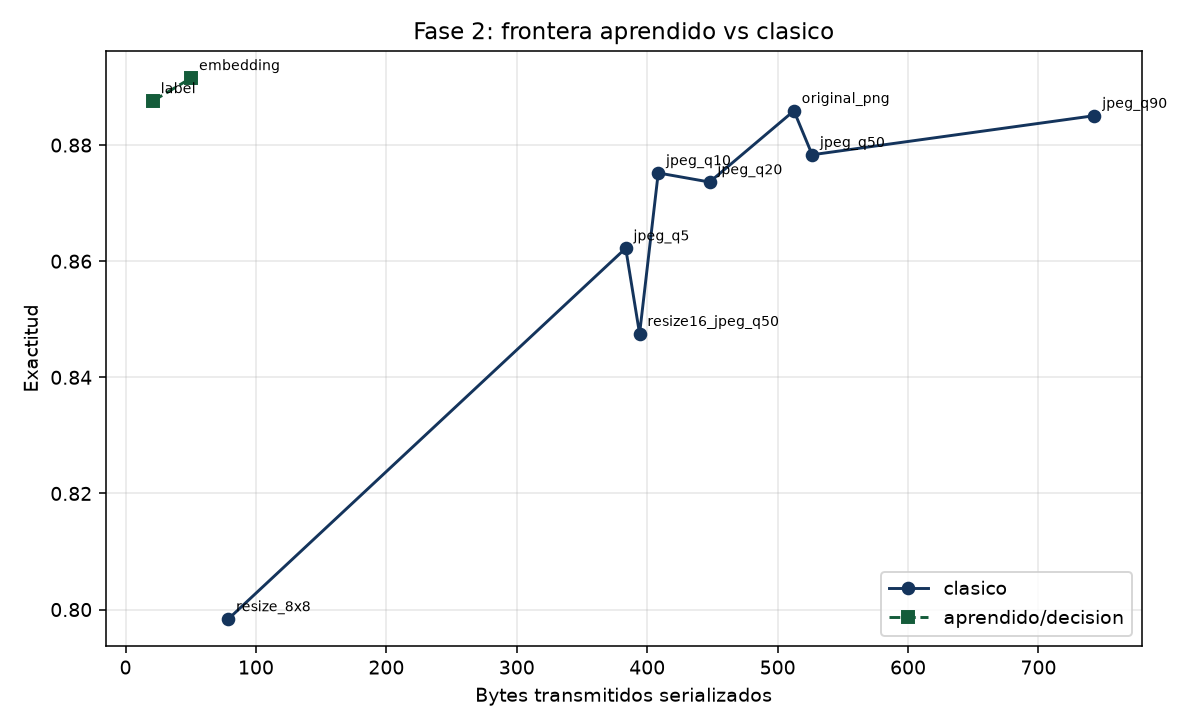
\includegraphics[width=0.82\linewidth]{results/figures/phase2_learned_vs_classic_frontier.png}
\caption{Fase 2: frontera aprendido vs. cl\'asico en Fashion-MNIST.}
\end{figure}

\textbf{Veredicto.} Bajo este protocolo y el cat\'alogo evaluado, el \emph{embedding} domina en Pareto a las representaciones cl\'asicas: obtiene mayor exactitud que los cl\'asicos con menos bytes. Entre los cl\'asicos que conservan utilidad dentro de $\eps=0{,}03$, JPEG q5 es el mejor por utilidad por byte, aunque entra en la tolerancia por poco (0{,}8622 frente a $U_{\max}\approx 0{,}8916$). El \emph{embedding} pesa 50{,}4 bytes y obtiene 0{,}8916 de exactitud; JPEG q5 pesa 383{,}5 bytes y obtiene 0{,}8622. La utilidad por byte del \emph{embedding} es aproximadamente 7{,}9 veces la de JPEG q5.

El caso \texttt{resize\_8x8} ilustra por qu\'e el veredicto exige conservar utilidad: aunque su utilidad por byte supera a la de los JPEG, su exactitud cae a 0{,}7984, fuera de la tolerancia. Por tanto, no se considera ganador.

% ==========================================================
\section{Fase 3: validaci\'on en CIFAR-10}

La Fase 3 repite la comparaci\'on en CIFAR-10, un banco de prueba m\'as complejo que Fashion-MNIST dentro de este estudio: color, texturas y fondos. Tambi\'en es un escenario m\'as favorable para JPEG que las im\'agenes 28$\times$28 en escala de grises. La corrida usa CIFAR-10 completo, 10 \'epocas, 3 semillas y CPU. La Tabla 3 y la Figura 3 resumen los resultados principales.

\begin{table}[t]
\centering\small
\caption{Fase 3 (CIFAR-10), filas seleccionadas.}
\begin{tabular}{@{}lrrr@{}}
\toprule
Representaci\'on & Bytes & Exactitud & Utilidad/byte\\
\midrule
original (PNG)        & 2267{,}7 & 0{,}7136 & 0{,}00031\\
JPEG q90              & 1106{,}2 & 0{,}6963 & 0{,}00063\\
JPEG q5               &  670{,}8 & 0{,}5732 & 0{,}00085\\
resize $8{\times}8$   &  211{,}7 & 0{,}5340 & 0{,}00252\\
\textbf{embedding}    &  \textbf{59{,}8} & \textbf{0{,}7200} & \textbf{0{,}01203}\\
etiqueta              &   21{,}0 & 0{,}7057 & 0{,}03360\\
\bottomrule
\end{tabular}
\end{table}

\begin{figure}[t]
\centering
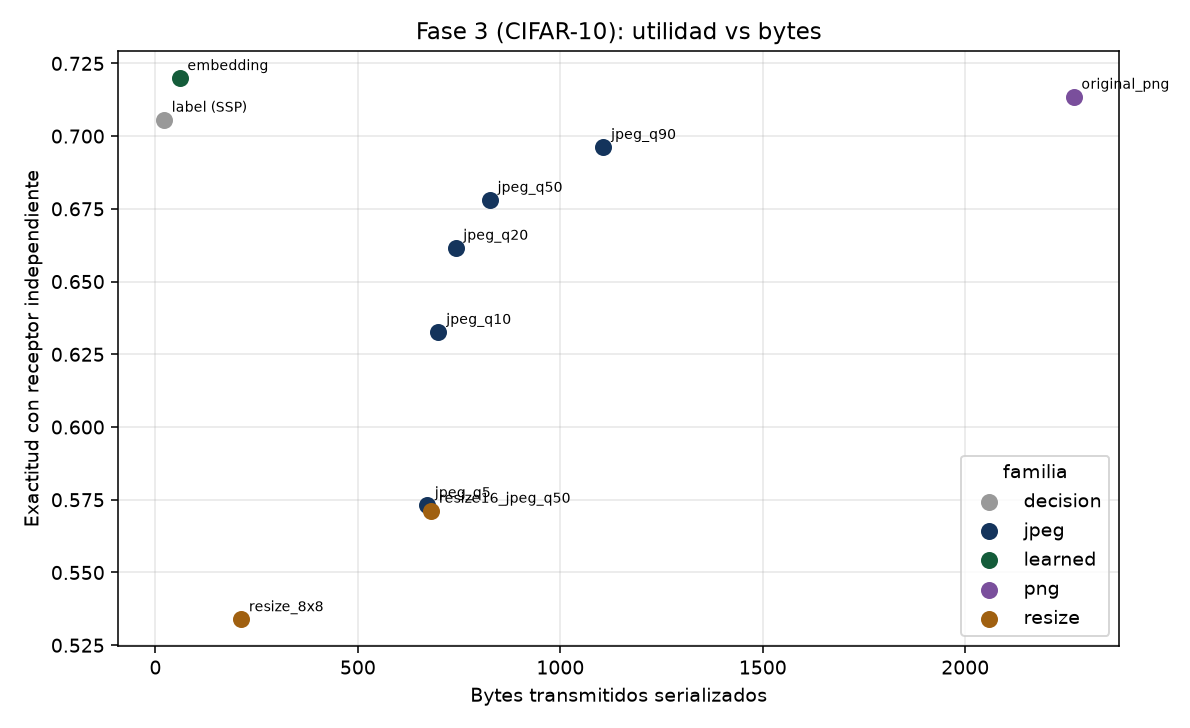
\includegraphics[width=0.82\linewidth]{results/figures/phase3_accuracy_vs_bytes.png}
\caption{Fase 3: utilidad vs. bytes en CIFAR-10, por familia de representaci\'on.}
\end{figure}

\textbf{Lectura.} El patr\'on observado en Fashion-MNIST persiste en CIFAR-10 bajo el protocolo evaluado: el \emph{embedding} conserva utilidad dentro de $\eps$ y pesa 59{,}8 bytes, frente a 2267{,}7 bytes del PNG original. El ahorro respecto al original sube de 90{,}2\% en Fashion-MNIST a 97{,}4\% en CIFAR-10. En estos dos bancos de prueba, la ventaja relativa del \emph{embedding} frente al mejor cl\'asico que conserva utilidad aument\'o: en CIFAR-10 el mejor cl\'asico dentro de $\eps$ es JPEG q90, con utilidad por byte 0{,}0006295; el \emph{embedding} alcanza 0{,}012034, una raz\'on aproximada de 19{,}1$\times$.

Esta observaci\'on no debe leerse como ley universal sobre fuentes complejas. Indica que, en estos dos bancos y con estos modelos, la representaci\'on orientada a tarea escal\'o mejor que las representaciones visuales evaluadas. Las exactitudes absolutas son menores que en Fashion-MNIST porque CIFAR-10 es m\'as dif\'icil y las CNN usadas son compactas.

% ==========================================================
\section{Fase 4: pol\'itica de transmisi\'on por umbral}

